\chapter{圖}

無向圖的節點定義如下:
\begin{Code}
// 無向圖的節點
struct UndirectedGraphNode {
    int label;
    vector<UndirectedGraphNode *> neighbors;
    UndirectedGraphNode(int x) : label(x) {};
};
\end{Code}


\section{Clone Graph} %%%%%%%%%%%%%%%%%%%%%%%%%%%%%%
\label{sec:clone-graph}


\subsubsection{描述}
Clone an undirected graph. Each node in the graph contains a \code{label} and a list of its \code{neighbours}.


OJ's undirected graph serialization:
Nodes are labeled uniquely.

We use \code{\#} as a separator for each node, and \code{,} as a separator for node label and each neighbour of the node.
As an example, consider the serialized graph \code{\{0,1,2\#1,2\#2,2\}}.

The graph has a total of three nodes, and therefore contains three parts as separated by \code{\#}.
\begin{enumerate}
\item First node is labeled as 0. Connect node 0 to both nodes 1 and 2.
\item Second node is labeled as 1. Connect node 1 to node 2.
\item Third node is labeled as 2. Connect node 2 to node 2 (itself), thus forming a self-cycle.
\end{enumerate}

Visually, the graph looks like the following:
\begin{Code}
       1
      / \
     /   \
    0 --- 2
         / \
         \_/
\end{Code}


\subsubsection{分析}
廣度優先遍歷或深度優先遍歷都可以。


\subsubsection{DFS}
\begin{Code}
// LeetCode, Clone Graph
// DFS,時間複雜度O(n),空間複雜度O(n)
class Solution {
public:
    UndirectedGraphNode *cloneGraph(const UndirectedGraphNode *node) {
        if(node == nullptr) return nullptr;
        // key is original node,value is copied node
        unordered_map<const UndirectedGraphNode *,
                            UndirectedGraphNode *> copied;
        clone(node, copied);
        return copied[node];
    }
private:
    // DFS
    static UndirectedGraphNode* clone(const UndirectedGraphNode *node,
            unordered_map<const UndirectedGraphNode *,
            UndirectedGraphNode *> &copied) {
        // a copy already exists
        if (copied.find(node) != copied.end()) return copied[node];

        UndirectedGraphNode *new_node = new UndirectedGraphNode(node->label);
        copied[node] = new_node;
        for (auto nbr : node->neighbors)
            new_node->neighbors.push_back(clone(nbr, copied));
        return new_node;
    }
};
\end{Code}


\subsubsection{BFS}
\begin{Code}
// LeetCode, Clone Graph
// BFS,時間複雜度O(n),空間複雜度O(n)
class Solution {
public:
    UndirectedGraphNode *cloneGraph(const UndirectedGraphNode *node) {
        if (node == nullptr) return nullptr;
        // key is original node,value is copied node
        unordered_map<const UndirectedGraphNode *,
                            UndirectedGraphNode *> copied;
        // each node in queue is already copied itself
        // but neighbors are not copied yet
        queue<const UndirectedGraphNode *> q;
        q.push(node);
        copied[node] = new UndirectedGraphNode(node->label);
        while (!q.empty()) {
            const UndirectedGraphNode *cur = q.front();
            q.pop();
            for (auto nbr : cur->neighbors) {
                // a copy already exists
                if (copied.find(nbr) != copied.end()) {
                    copied[cur]->neighbors.push_back(copied[nbr]);
                } else {
                    UndirectedGraphNode *new_node =
                            new UndirectedGraphNode(nbr->label);
                    copied[nbr] = new_node;
                    copied[cur]->neighbors.push_back(new_node);
                    q.push(nbr);
                }
            }
        }
        return copied[node];
    }
};
\end{Code}


\subsubsection{相關題目}
\begindot
\item 無
\myenddot

\section{Network Delay Time} %%%%%%%%%%%%%%%%%%%%%%%%%%%%%%
\label{sec:network-delay-time}


\subsubsection{描述}
There are N network nodes, labelled 1 to N.

Given times, a list of travel times as directed edges times[i] = (u, v, w), where u is the source node, v is the target node, and w is the time it takes for a signal to travel from source to target.

Now, we send a signal from a certain node K. How long will it take for all nodes to receive the signal? If it is impossible, return -1.

\begin{center}
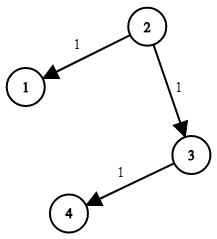
\includegraphics[width=100pt]{network-delay-time.png}\\
\figcaption{Rotate Image}\label{fig:network-delay-time}
\end{center}

\begin{Code}
Input: times = [[2,1,1],[2,3,1],[3,4,1]], N = 4, K = 2
Output: 2
\end{Code}

\begin{enumerate}
\item N will be in the range [l, 100]
\item K will be in the range [l, N]
\item The length of times will be in the range [l, 6000].
\item All edges times[i] = (u, v, w) will have l <= u, v <= N and 0 <= w <= 100.
\end{enumerate}
\subsubsection{分析}
廣度優先遍歷
Use Djikstra Algorithm. Find a minium path from one source to one end.


\subsubsection{Djikstra}
\begin{Code}
// LeetCode, Clone Graph
// DFS with graph,時間複雜度O(ELogV),空間複雜度O(V^2)
class Solution {
public:
    struct Node {
        int m_node;
        int m_dist;

        Node (int node, int dist)
            : m_node(node), m_dist(dist) {}
    };
    int networkDelayTime(vector<vector<int>>& times, int N, int K) {
        // create graph
        unordered_map<int, list<Node>> graph;  // key: nodeNumber value: nodes
        for (const auto& t : times) // startNode: t[0], endNode: t[1], dist: t[2]
            graph[t[0]].push_back(Node(t[1], t[2]));

        unordered_map<int, int> dist; // key: nodeNumber value: dist
        multimap<int, int> dq; // djikstra queue, key: dist value: nodeNumber

        // do until no more node in queue
        dq.insert(make_pair(0, K));
        while (!dq.empty()) {
            pair<int, int> cur = *dq.begin();
            dq.erase(dq.begin());

            // filter out if shortest path is found
            if (dist.find(cur.second) != dist.end()) continue;
            // record the shortest parth
            dist.insert(make_pair(cur.second, cur.first));
            // push the neighbour to dq
            auto it = graph.find(cur.second);
            if (it == graph.end()) continue;
            for (const auto& nei : it->second) {
                if (dist.find(nei.m_node) != dist.end()) continue;
                dq.insert(make_pair(nei.m_dist + cur.first, nei.m_node));
            }
        }

        // pick the max dist, return -1 if not all node is visited
        if ((int)dist.size() == N)
            return max_element(dist.begin(), dist.end()
              , [&](const pair<int, int>& first, const pair<int, int>& second)
                                {
                                    return first.second < second.second;
                                })->second;
        else
            return -1;
    }
};

\end{Code}
\subsubsection{Djikstra}
\begin{Code}
// LeetCode, Clone Graph
// DFS with adjacency list,時間複雜度O(ELogV),空間複雜度O(V^2)
class Solution {
public:
    int networkDelayTime(vector<vector<int>>& times, int N, int K)
    {
        // Build adjacency list
        // index 0 is dummy for easy implementation
        vector<vector<pair<int, int>>> adjList(N + 1);
        for (const auto& v : times)
            adjList[v[0]].emplace_back(v[1], v[2]);

        vector<int> dist(N + 1, INT_MAX);
        // initialize pq and source vertex distance
        dist[K] = 0;
        set<pair<int, int>> pq {{dist[K], K}};
        while (!pq.empty()) {
            const auto u = pq.begin()->second;
            pq.erase(pq.begin()); // pop the top, i.e., first element in set
            for (const auto& [v, w]: adjList[u]) {
                if (dist[u] + w < dist[v]) { // if edge can be relaxed
                    pq.erase({dist[v], v}); // remove old info
                    dist[v] = dist[u] + w;  // update distance
                    pq.emplace(dist[v], v); // insert new info
                }
            }
        }

        const int longestTime = *max_element(dist.begin() + 1, dist.end());
        return longestTime == INT_MAX ? -1 : longestTime;
    }
};
\end{Code}

\subsubsection{相關題目}
\begindot
\item 無
\myenddot

\section{Alien Dictionary} %%%%%%%%%%%%%%%%%%%%%%%%%%%%%%
\label{sec:alien-dictionary}

\subsubsection{描述}
There is a new alien language which uses the latin alphabet. However, the order among letters are unknown to you. You receive a list of non-empty words from the dictionary, where words are sorted lexicographically by the rules of this new language. Derive the order of letters in this language.

Example 1:
\begin{Code}
Input:
[
  "wrt",
  "wrf",
  "er",
  "ett",
  "rftt"
]

Output: "wertf"
\end{Code}

Example 2:
\begin{Code}
Input:
[
  "z",
  "x"
]

Output: "zx"
\end{Code}

Example 3:
\begin{Code}
Input:
[
  "z",
  "x",
  "z"
] 

Output: "" 
\end{Code}

\subsubsection{分析}
Make DAG from sorted strings, do topological sort by BFS or DFS


\subsubsection{BFS with List}
\begin{Code}
// LeetCode, Alien Dictionary
// BFS Topological sort,時間複雜度O(N),空間複雜度O(N)
class Solution {
public:
    string alienOrder(vector<string>& words) {
        unordered_map<char, list<char>> adjList; // 用來記低依賴關係
        unordered_map<char, int> depenCount; // 用來儲存每個字母的依賴數目

        for (const auto& w : words)
            for (const auto& c : w)
            {
                depenCount[c] = 0;
                adjList.insert(make_pair(c, list<char>()));
            }
        // 製造 adjList DAG
        for (size_t i = 0; i < words.size() - 1; i++)
        {
            const string& w1 = words[i];
            const string& w2 = words[i+1];
            // 剪枝,若 prefix 一樣
            if (w1.size() > w2.size() && w1.find(w2) == 0) return "";
            // 找尋第一個不同的字母
            for (size_t j = 0; j < w1.size() && j < w2.size(); j++)
            {
                const char& c1 = w1[j];
                const char& c2 = w2[j];
                if (c1 != c2)
                {
                    adjList[c1].push_back(c2);
                    depenCount[c2]++;
                    break;
                }
            }
        }
        // 利用 Topological Sort 來解決相關的依賴關係
        queue<char> cur;
        // 先處理沒有依賴的字母
        for (const auto& [k, v] : depenCount)
            if (v == 0)
                cur.push(k);

        string result;
        // BFS
        while (!cur.empty())
        {
            char c = cur.front();
            cur.pop();
            result.push_back(c);
            auto it = adjList.find(c);
            if (it == adjList.end()) continue;
            for (const auto& nei : it->second)
            {
                if (--(depenCount[nei]) == 0)
                    cur.push(nei);
            }
        }

        if (result.size() < depenCount.size())
            return "";
        else
            return result;
    }
};
\end{Code}

\subsubsection{BFS with Set}
\begin{Code}
// LeetCode, Alien Dictionary
// BFS Topological sort,時間複雜度O(N),空間複雜度O(N)
class Solution {
public:
    string alienOrder(vector<string>& words) {
        unordered_map<char, set<char>> adjList; // 用來記低依賴關係
        unordered_map<char, int> depenCount; // 用來儲存每個字母的依賴數目

        for (const auto& w : words)
            for (const auto& c : w)
            {
                depenCount[c] = 0;
                adjList.insert(make_pair(c, set<char>()));
            }
        // 製造 adjList DAG
        for (size_t i = 0; i < words.size() - 1; i++)
        {
            const string& w1 = words[i];
            const string& w2 = words[i+1];
            // 剪枝,若 prefix 一樣
            if (w1.size() > w2.size() && w1.find(w2) == 0) return "";
            // 找尋第一個不同的字母
            for (size_t j = 0; j < w1.size() && j < w2.size(); j++)
            {
                const char& c1 = w1[j];
                const char& c2 = w2[j];
                if (c1 != c2)
                {
                    if (adjList[c1].find(c2) == adjList[c1].end()) // 這裏不同
                    {
                        adjList[c1].insert(c2);
                        depenCount[c2]++;
                    }
                    break;
                }
            }
        }
        // 之後的動作和上一個例子一樣,略去 。。。 //
    }
};

\end{Code}

\subsubsection{DFS with List}
\begin{Code}
// LeetCode, Alien Dictionary
// DFS Topological sort,時間複雜度O(N),空間複雜度O(N)
class Solution {
public:
    string alienOrder(vector<string>& words) {
        unordered_map<char, list<char>> adjList; // 用來記低依賴關係
        
        // 製造 DAG,令到所有字母也有被歷篇的機會
        for (const auto& w : words)
            for (const auto& c : w)
                adjList.insert(make_pair(c, list<char>()));
        // 製造剩下的 DAG
        for (size_t i = 0; i < words.size() - 1; i++)
        {
            const string& w1 = words[i];
            const string& w2 = words[i+1];
            // 找到 prefix case
            if (w1.size() > w2.size() && w1.find(w2) == 0) return "";
            
            for (size_t j = 0; j < w1.size() && j < w2.size(); j++)
            {
                const char& c1 = w1[j];
                const char& c2 = w2[j];
                if (c1 != c2)
                {
                    adjList[c1].push_back(c2);
                    break;
                }
            }
        }
        
        string result;
        unordered_map<char, bool> visited;
        for (const auto& [k, v] : adjList)
        {
            if (!DFS(adjList, visited, k, result))
                return "";
        }
        
        if (result.size() < adjList.size())
            return "";
        else
            return result;
    }
private:
    bool DFS(unordered_map<char, list<char>>& adjList, unordered_map<char, bool>& visited, char k, string& result)
    {
        if (visited.find(k) != visited.end())
            return visited[k]; // If this node was grey (false), a cycle was detected.
        
        visited[k] = false;
        auto it = adjList.find(k);
        for (const auto& nei : adjList[k])
        {
            if (!DFS(adjList, visited, *nei, result)) return false;
        }
        visited[k] = true;
        result.insert(result.begin(), k);
        
        return true;
    }
};

\end{Code}

\subsubsection{相關題目}
\begindot
\item Topological sort,見 \S \ref{sec:topological-sort}
\myenddot

\section{Redundant Connection} %%%%%%%%%%%%%%%%%%%%%%%%%%%%%%
\label{sec:redundant-connection}

\subsubsection{描述}
In this problem, a tree is an undirected graph that is connected and has no cycles.

The given input is a graph that started as a tree with N nodes (with distinct values 1, 2, ..., N), with one additional edge added. The added edge has two different vertices chosen from 1 to N, and was not an edge that already existed.

The resulting graph is given as a 2D-array of edges. Each element of edges is a pair [u, v] with u < v, that represents an undirected edge connecting nodes u and v.

Return an edge that can be removed so that the resulting graph is a tree of N nodes. If there are multiple answers, return the answer that occurs last in the given 2D-array. The answer edge [u, v] should be in the same format, with u < v.


Example 1:
\begin{Code}
Input: [[1,2], [1,3], [2,3]]
Output: [2,3]
Explanation: The given undirected graph will be like this:
  1
 / \
2 - 3
\end{Code}

Example 2:
\begin{Code}
Input: [[1,2], [2,3], [3,4], [1,4], [1,5]]
Output: [1,4]
Explanation: The given undirected graph will be like this:
5 - 1 - 2
    |   |
    4 - 3
\end{Code}


Note:
\begindot
\item The size of the input 2D-array will be between 3 and 1000.
\item Every integer represented in the 2D-array will be between 1 and N, where N is the size of the input array.
\myenddot


\subsubsection{DFS}
\begin{Code}
// 時間複雜度O(N^2),空間複雜度O(N)
// 重點:當發現有多過一個路徑可由 u 走到 v,便發現答案
class Solution {
public:
    vector<int> findRedundantConnection(vector<vector<int>>& edges) {
        // 記低見過的 edges, 由 u -> v
        unordered_map<int, unordered_set<int>> cache;

        for (const auto& edge : edges)
        {
            const int& u = edge[0];
            const int& v = edge[1];
            // 利用 DFS 來驗證有沒有另一個方法可以由 u 跑到 v
            unordered_set<int> visited;
            if (cache.count(u) && cache.count(v) && DFS(cache, visited, u, v))
                return vector<int>{u, v};

            cache[u].insert(v);
            cache[v].insert(u);
        }

        return vector<int>();
    }
private:
    template <class eMap, class Vis>
        bool DFS(eMap& cache, Vis& visited, const int& start, const int& target)
    {
        if (start == target) return true;

        if (cache.find(start) == cache.end()) return false;

        visited.insert(start);
        for (const int& nei : cache[start])
            if (!visited.count(nei) && DFS(cache, visited, nei, target))
                return true;

        return false;
    }
};
\end{Code}

\subsubsection{DSU - Without Rank}
\begin{Code}
// 時間複雜度O(N),空間複雜度O(N)
// 一開始每個點都以自己為一個集合(set)
// 歷遍所有 edge,把點放於同一個集合。
// 若果兩點早已是同一集合,那個 edge 便是多餘。
// https://www.youtube.com/watch?time_continue=1124&v=wU6udHRIkcc&feature=emb_title
class DSU // Disjoint Set Union (DSU)
{
public:
    DSU(int N)
    {
        m_parent.reserve(N);
        for (int i = 0; i < N; i++) m_parent.push_back(i);
    }
    ~DSU() {}

    int FindParent(const int& x)
    {
        if (m_parent[x] == x) // 當 x 為集合的父親時
            return x;
        return m_parent[x] = FindParent(m_parent[x]); // x 的集合等如 x 的父親的集合
    }
    bool Union(const int& x, const int& y)
    {
        const int xpar = FindParent(x);
        const int ypar = FindParent(y);
        if (xpar == ypar) return false;

        m_parent[xpar] = ypar; // perform union

        return true;
    }
private:
    vector<int> m_parent; // 利用數列來記低點的所在集合
};
class Solution
{
public:
    vector<int> findRedundantConnection(vector<vector<int>>& edges) {
        DSU dsu(1001);

        for (const auto& edge : edges)
        {
            const int& u = edge[0];
            const int& v = edge[1];

            if (!dsu.Union(u, v))
                return vector<int>{u, v};
        }

        return vector<int>();
    }
};
\end{Code}

\subsubsection{DSU - Rank}
\begin{Code}
// 時間複雜度O(N),空間複雜度O(N)
// 一開始每個點都以自己為一個集合(set)
// 歷遍所有 edge,把點放於同一個集合。
// 若果兩點早已是同一集合,那個 edge 便是多餘。
class DSU // Disjoint Set Union (DSU)
{
public:
    DSU(int N)
    {
        // 負數意指該合集的父親
        // 所以一開始,每個點都是某個合集的父親
        // 負數的值代表 rank, 也是該合集的點的總數
        // 正數的值代表父的 index
        m_parent.resize(N, -1);
    }
    ~DSU() {}

    int FindParent(const int& x)
    {
        if (m_parent[x] < 0)
            return x;
        return m_parent[x] = FindParent(m_parent[x]);
    }
    bool Union(const int& x, const int& y)
    {
        const int xpar = FindParent(x);
        const int ypar = FindParent(y);
        if (xpar == ypar) return false;

        if (abs(m_parent[xpar]) < abs(m_parent[ypar]))
        {
            m_parent[ypar] += m_parent[xpar];
            m_parent[xpar] = ypar;
        }
        else
        {
            m_parent[xpar] += m_parent[ypar];
            m_parent[ypar] = xpar;
        }

        return true;
    }
private:
    vector<int> m_parent;
};
class Solution {
public:
    vector<int> findRedundantConnection(vector<vector<int>>& edges) {
        DSU dsu(1001);

        for (const auto& edge : edges)
        {
            const int& u = edge[0];
            const int& v = edge[1];

            if (!dsu.Union(u, v))
                return vector<int>{u, v};
        }

        return vector<int>();
    }
};
\end{Code}
